\namedsection{FPGA}{Pasat}

\subsection{Introduction}

A FPGA (field-programmable gate array) is an semiconductor device which is has a matrix of CLBs (configurable logic blocks) connected through programmable interconnects. One main advantage of FPGAs is that the can be preprogrammed after they are manufactured in order to fit desired functionalities and requirements, such as the ones required by our team's project.
\\\\
The two devices we are using, the FPGA and the Microcontroller, are two very different devices. The microcontroller has the chip already designed. The programmer simply writes the software in C or C++, then it is compiled into a hex file that is loaded on the microcontroller. The program is stored in the flash memory until is is replaced or erased.
\\\\
FPGAs are different in this sense. The circuit is completely designed by the programmer. The processor must be created and can be as simple as an and gate or can be our Cortex M0+. HDL is used to write the design, which is then synthesized into a bit file which configures the FPGA. One small problem with this is the fact that it stores the configuration in the RAM, so once the power is gone, the configuration is lost.
\\\\\
The board used for this project is the Xilinx Digilent Nexys4, which can be seen in figure \ref{figure: nexys4} on the next page. It is based on the Artix-7 that has the lowest power consumption at 28nm and is optimized to give the design the highest performance. We chose this board because it is a large, high-capacity FPGA board that would be sufficient for our project. Another reason is the fact that is has several built in peripherals, such as accelerometer, which would be useful for the exercise detection. 
\begin{figure}
\centering
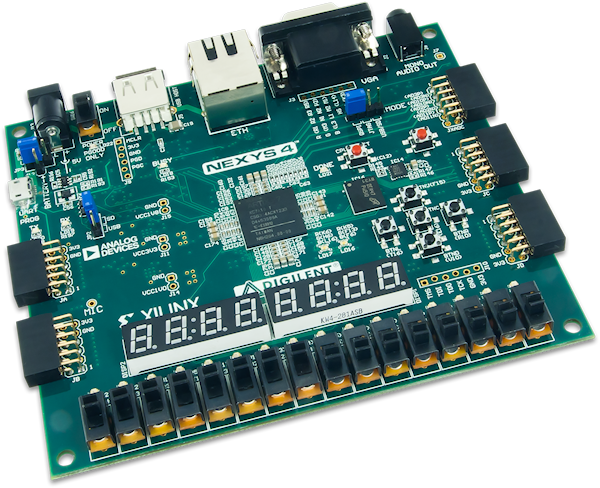
\includegraphics[scale=0.7]{figures/nexys4.PNG}
\caption{Xilinx Digilent Nexys4 \label{fig:nexys4}}
\end{figure}

Next,the implementation of the Cortex M0 DesignStart on the FPGA board will be discussed. The system will have a Cortex-M0\_DS processor, a preloaded memory with a program that fetches constants from a memory at regular intervals, a reset and a pattern detector attached to the bus so when a specific pattern appears on the data bus, the LED turns on and when another patters appears it will turn off. The Cortex-M0\_DS  includes only the processor a non-synthesizable testbench. Other parts will need to be implemented in order to create an synthesizable system: a software executable image, a memory holding the program, a system clock, a detector module for the command LED and a reset synchronizer. This section will be divided into: software development and simulation, system implementation and functional simulation. All of these sections will be discussed in detail in what follows.

\subsection{Software development and simulation}
In this section, a software program that will verify the memory fetches of some predefined constants. The program used for this will be ARM Keil μVision, which is a IDE(Integrated Development Environment) which allows quick and easy building of projects and includes other facilities such as: make facilities, source code debug, program debug and complete simulations.

To start, a new project must be created in μVision. Next, the device must be selected device database so ARM-ARM Cortex M0 plus-ARMCM0P is selected which can be seen in figure \ref{armcm0p}.
\begin{figure}
\centering
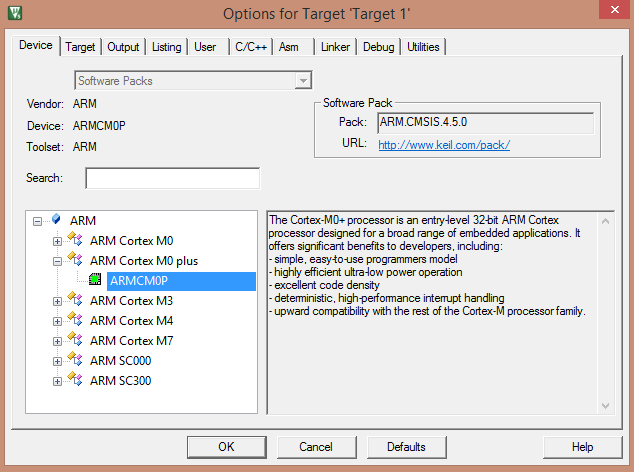
\includegraphics[scale=0.7]{figures/armcm0p.PNG}
\caption{Selection of the Cortex M0+ for the μVision project} 
\label{fig:armcm0p}
\end{figure}

After this is selected, the options menu is accessed for this device. Next, the target options need to be accessed and the following modification need to be made:

- under Target section, the Read/Write Memory Areas, RAM1 starts at 0x0 and has the size of 0x400000 (this setting is used to create a linker scatter file. Another requirement for this is the having the Use Memory Layout from Target Dialog enabled in the Linker section);

- under Output section, the Debug Information and Browse Information sections need to be ticked(this defines the resulting output files from the tool chain and allows the user programs to be started after the building process is complete);

- under Listing section, all the default selected features stay the same(here all the listing files generated by the tool chain are specified);

- under User section, in Run\#1:"fromelf -cvf code.axf --vhx --32x1 -o code.hex" and Run\#2:"fromelf -cvf code.axf -o disasm.txt" in Run User Programs After Build/Rebuild those code lines are inserted in order to create a .axf file from the .hex file;

- under C/C++ section, the One ELF Section per Function is unticked and the Warnings are set to <unspecified> (here C/C++ specific tool options are set);

-under Asm section, all the settings are kept to default also( this allows the setting of specific Assembler tool options);

-under Linker section, the R/W Base entry is deleted and only the R/O Base: 0x00000000 remains(linker settings are required in order to configure the physical memory location of the target). The location of memory classes and sections is defined here.

-under Debug section, the default settings for µVision4 Debugger stay the same;

-under Utilities, the Use Target Driver for Flash Programming in the Configure Flash Menu Command is left checked.

After all of these steps have been done,it is now time to add assembly file provided by ARM, the cm0dasm.s to the source. Taking a look at the reset handler, which can be seen in \ref{reset_handler},  the value 0x55 is written to the LED when a specific pattern is detected and 0xAA if another pattern is detected.
\begin{figure}
\centering
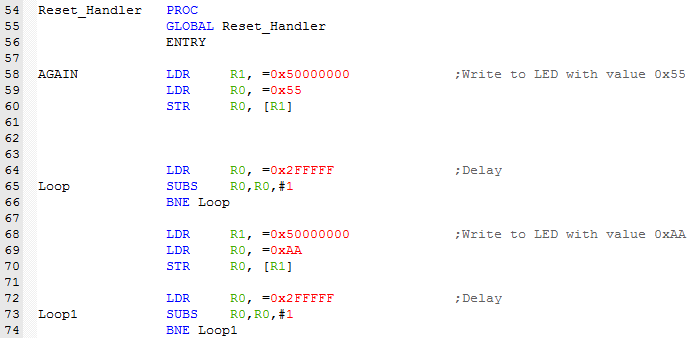
\includegraphics[scale=0.7]{figures/reset_handler.PNG}
\caption{Reset handler} 
\label{fig:armcm0p}
\end{figure}

After the successful building of the code.hex should be created and converted into a .axf because it was set in the User section. The .axf file needs to be converted to a .bin in order to program the FPGA. The MDK/Keil offers a tool called "fromelf" which can do this conversion. It is called in the following way:

fromelf --bin --o code.bin code.axf

This can be ued to program the FPGA. Now, the implementation of the Cortex-M0+ will be discussed.

\subsection{System Implementation}

ARM offers access to packs that makes the implementation of the Cortex M0+ on the FPGA is discussed. The components which will be used are: the ARM Cortex-M0 processor, the AHB-Lite system bus and two AHB peripherals: the program memory(which will be implemented using on-chip memory blocks) and a simple LED peripheral.

The software used for this implementation is Vivado Design Suite. This software is produced by Xilinx and is used for synthesis and analysis of HDL designs and is a improved version of the Xilinx ISE which also allows features such as system on a chip development and a high-level synthesis. A new project must be created

The ARM DesignStart  package which contains the logic of the ARM Cortex-M0 processor written in Verilog and can be synthesized and implemented on a FPGA platform. The Cortex-M0 DesignStart will be used, which is a simplified version of the industry Cortex-M0 processor, but has some features reduced which are not essential for this project such as in the number of interrupts(from 32 to 16). Two verilog files are included in this pack:  cortexm0ds\_logic.v and CORTEM0DS.v. The cortexm0ds\_logic.v contains the Cortex-M0 DesignStart processor logic level Verilog file, while the CORTEXM0DS.v includes the Cortex-M0 DesignStart processor macro cell level.

The software code needs to be compiled to machine code in order to program the processor.